\begin{figure}
		\begin{center}		
	
	\subfloat{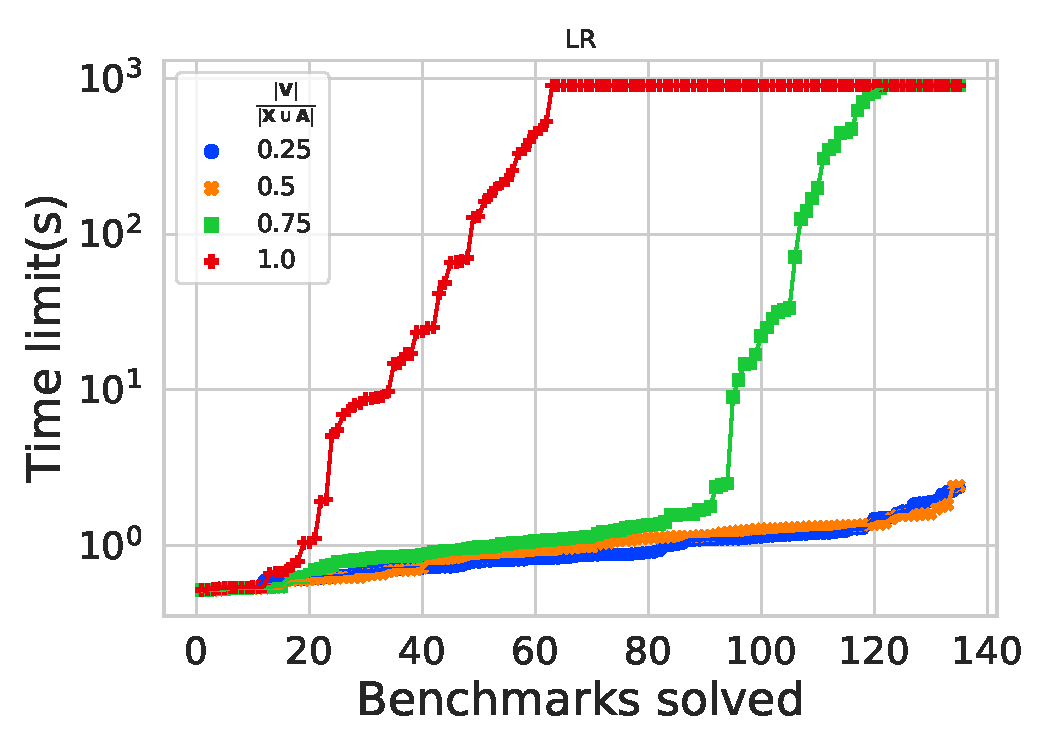
\includegraphics[scale=0.4]{figures/fairness/fvgm/cactus_dag_LR_time}}
	\subfloat{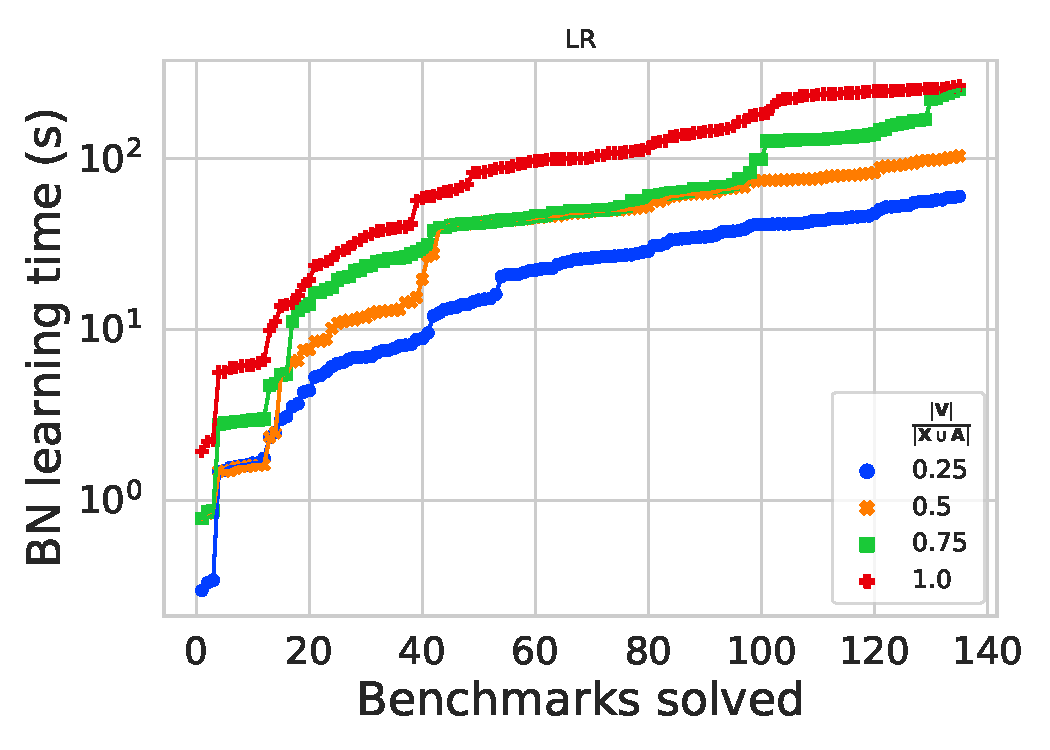
\includegraphics[scale=0.4]{figures/fairness/fvgm/cactus_dag_LR_time_notears}}
			
		\end{center}
		
		\caption{Effect of number of variables in the learned Bayesian Network on computation time of {\fvgm}. In both plots, we vary $ \frac{|\mathbf{V}|}{|\nonsensitive \cup \sensitive|} $, that is the ratio between the number of variables in the Bayesian Network to the number of features. We observe that as this ratio increases to $ 1 $, both runtime of {\fvgm} (left plot) and network learning time (right plot) increase. } 
		\label{fairness_fvgm_fig:results_DAG_complexity}
\end{figure}
	
	
	
